\documentclass[PICOReport.tex]{subfiles}

\begin{document}

%\noindent{\bf Introduction} \\
Observations of Galactic polarization are a highlight and a lasting legacy of the {\em Planck} space mission. 
Spectacular images combining the intensity of dust with the texture derived from polarization data 
have received world-wide attention and have become part of the general scientific culture \citep{PlanckI2015}. 
Beyond their popular impact, the Planck polarization maps represented an 
immense step forward for Galactic astrophysics \citep{Planck2018:XII}. 
We expect an even greater leap forward from PICO based on the higher angular resolution dust polarization images obtained with the balloon experiment BLASTPol.  
PICO will provide all-sky maps of dust polarization at higher resolution than BLASTPol and with significantly higher sensitivity than {\em Planck}. Such a data set can only be obtained from a space mission. Planck made hundreds of thousands of measurements of magnetic field orientation across the sky; with PICO we expect $\sim1.5\times 10^8$ independent measurements in the 799 GHz band alone.
The data will complement a rich array of polarization observations including stellar polarization surveys to be 
combined with Gaia astrometry and synchrotron observations measuring Faraday rotation at radio wavelengths 
with the Square Kilometer Array and its precursors. 
In this section we focus on two key crucial Galactic science measurements that only PICO can obtain.

(1) {\em Testing Composition Models of Interstellar Dust:}
The analysis of the PICO data will involve the spectral characterization of Galactic polarization. 
This aspect of the data analysis will continue to update and test models of dust emission and of grain alignment, which are of interest for the interpretation of dust polarization data at large.


(2) {\em Determining how magnetic fields affect the processes of molecular cloud and star formation:}
By virtue of the strong dynamical coupling of dust and gas and the systematic alignment of dust grains with magnetic fields, dust polarization probes magnetic fields in 
the cold and warm neutral phases of the ISM and in molecular gas.
If the magnetic fields are sufficiently strong, they can prevent the gravitational collapse of gas across magnetic field lines and can slow down or limit the processes of star and planet formation.
In the diffuse ISM the neutral phase of the interstellar medium contains the bulk of the gas mass 
and of its turbulent kinetic energy.\vspace{0.1in} \\
%
%
\begin{figure}
    \centering
    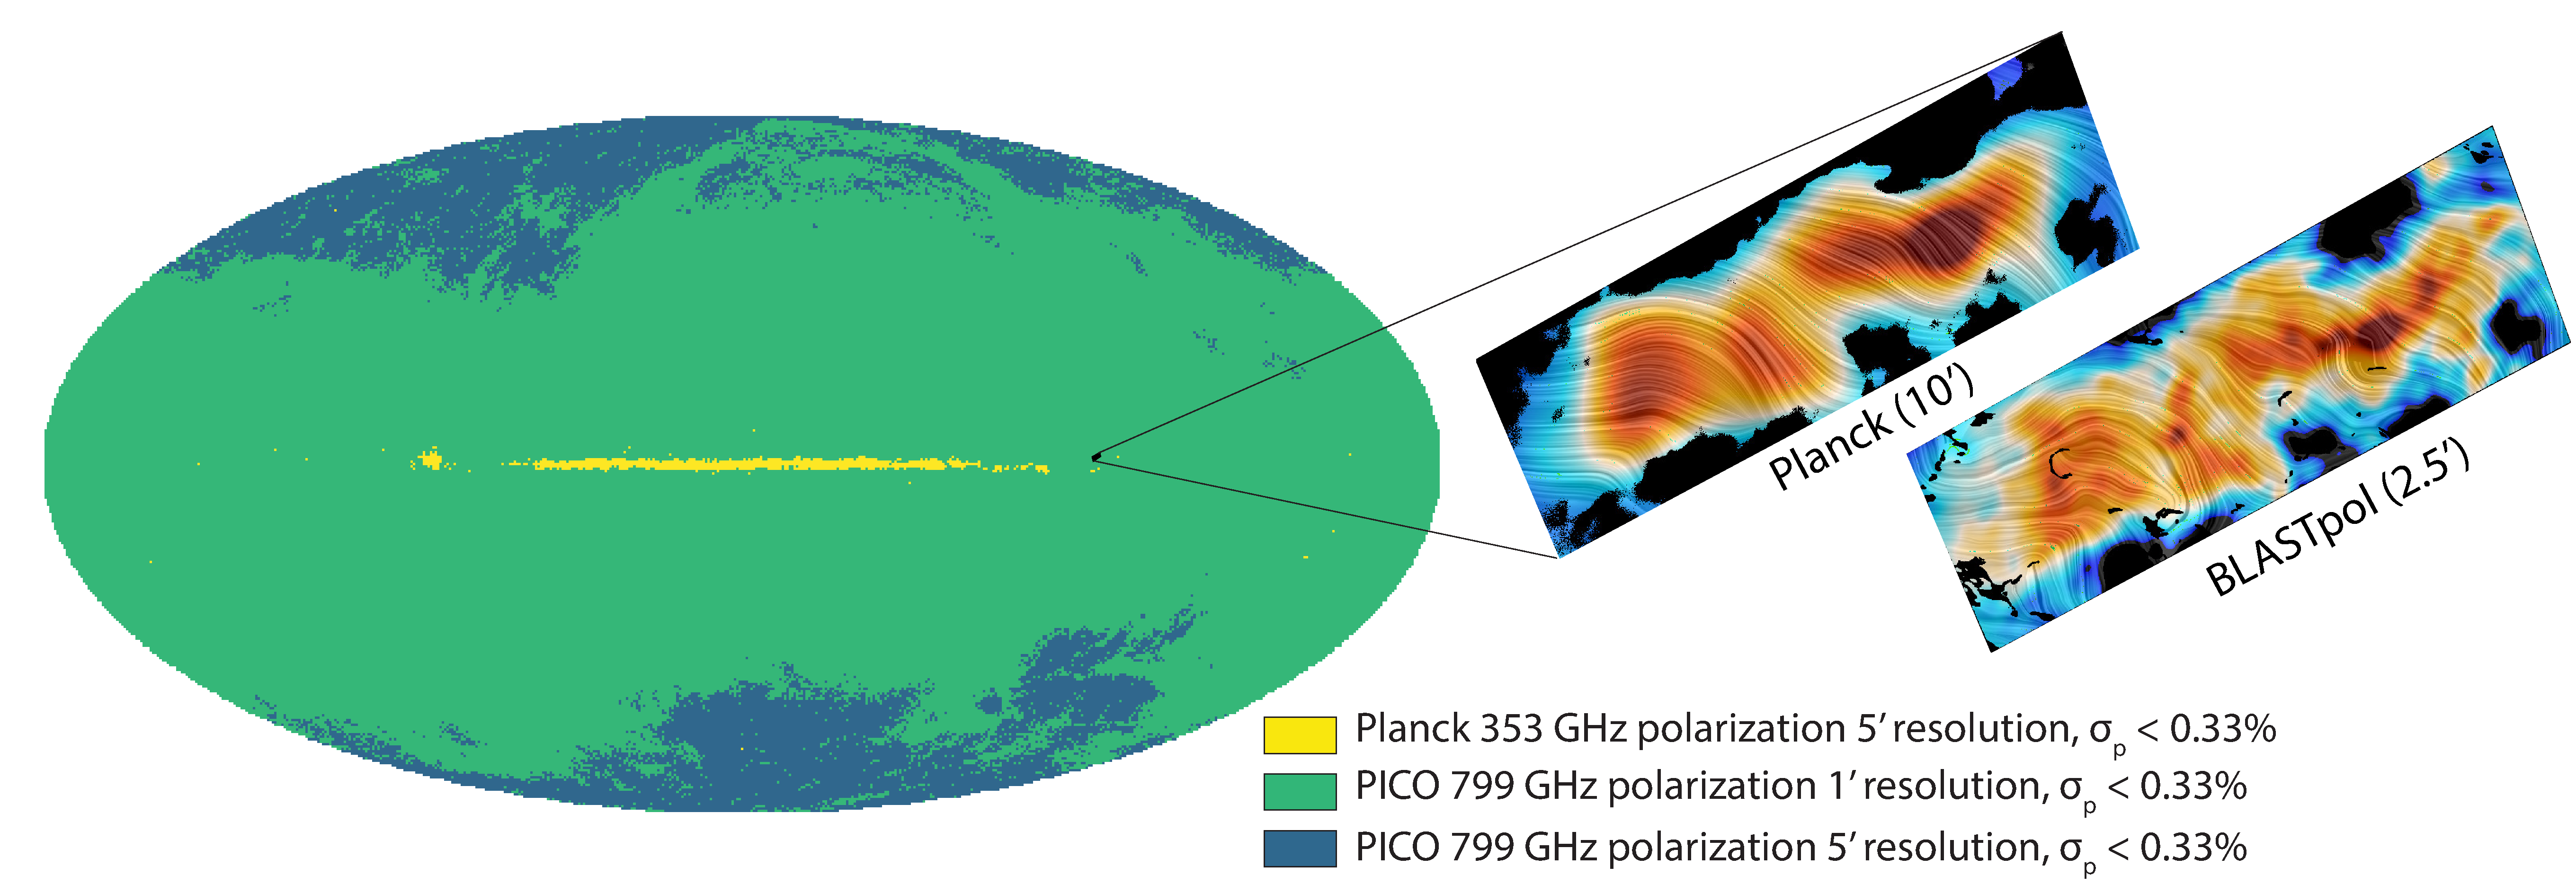
\includegraphics[width=6in]{galsci_fig.pdf}
    \caption{At 799 GHz, the PICO Baseline mission will map nearly the entire sky at 1$^{\prime}$ resolution. As an example of the current state-of-the-art, Planck (10$^{\prime}$) and BLASTpol (2.5$^{\prime}$) maps of the Vela C region are shown \citep{Fissel2016}. These observations will enable PICO to characterize magnetized turbulence from the diffuse ISM down to dense star forming cores.}
    \label{fig:allsky}
\end{figure}
%
%
{\bf Dust Physics} \\
Strong extinction features at 9.7 and 18\,$\mu$m indicate much interstellar dust is in the form of amorphous silicates while features at 2175\,\AA, 3.3\,$\mu$m, and 3.4\,$\mu$m attest to abundant hydrocarbons. It is unknown, however, whether the silicate and carbonaceous materials coexist on the same grains or whether they are segregated into distinct grain populations. If there are indeed multiple grain species, this will induce additional challenges for modeling the emission from interstellar dust in both total intensity and polarization at levels relevant for B-mode science \citep{Hensley2018}.

Spectropolarimetry of dust extinction features reveals robust polarization in the 9.7\,$\mu$m silicate feature \citep[e.g.,][]{Smith2000}, indicating that the silicate grains are aligned with the interstellar magnetic field. In contrast, searches for polarization in the 3.4\,$\mu$m carbonaceous feature have yielded only upper limits, even along sightlines where silicate polarization is observed \citep{Chiar2006,Mason2007}. These data suggest that most of the silicate and carbonaceous materials do not exist on the same grains. However, these studies are limited to only a few highly-extincted sightlines that may not typify the diffuse ISM.

At odds with the spectropolarimetric evidence from dust extinction, current measurements of the polarization fraction of the far-infrared dust emission with {\it Planck} \citep{Planck_Int_XXII} and BLASTPol \citep{Ashton2018} betray little to no frequency dependence, as would be expected if two components with distinct polarization properties were contributing to the total emission. However, current uncertainties are relatively large and the data with $\nu > 353\,$GHz are from high density sightlines that may not be representative of the diffuse ISM. With great polarization sensitivity even in diffuse regions, PICO will provide a definitive test of the two component paradigm.

To assess PICO's ability to discriminate quantitatively, we employ the analytic two component dust mode of \cite{Meisner2015} which provided a better fit to IRAS and {\it Planck} data than one component models. 

Applying the noise estimates from PICO, 1000 simulations were run for different combinations of polarization fractions of the two components in this model. Only frequency channels 107 GHz and above were used, and the simulated data were binned to the 7.9$^\prime$ beam of PICO?s 107 GHz channel. Based on the variance of the simulation results, PICO can determine the intrinsic polarization fractions of the two components to a precision of 1-2\%. PICO will therefore be able to validate or reject state-of-the-art dust models \citep[e.g.][Hensley \& Draine, in prep]{Guillet2018} and test for the presence of additional grain species with distinct polarization signatures, such as magnetic nanoparticles \citep{Draine2013}.%
%
\noindent{\bf Are Magnetic Fields Responsible For Low Star Formation Efficiency?} \\
Stars form out of dense, gravitationally unstable regions within molecular gas clouds. The efficiency of this conversion from molecular gas to stars is very low, due to regulation from supersonic turbulent gas motions, magnetic fields, and feedback from young stars \citep{McKee2007}. 
Magnetic fields may play an important role in slowing the process of star formation by inhibiting movement of gas in the direction perpendicular to the field lines.  Observations to date suggest that the outer envelopes of clouds can be supported against gravity by magnetic fields, but in dense cores gravity tends to dominate, and so these dense structures can collapse to form stars \citep{Crutcher2010}.

On larger scales, the formation of gravitationally unstable clouds is regulated by the flow of diffuse material into the molecular phase, a process that is mediated by magnetized turbulence in the low-density ISM. Structure formation in the diffuse ISM is poorly understood, but as a precursor to star formation it is crucial to understand what drives molecular cloud formation. Recent observations suggest that the structure of the diffuse medium is highly anisotropic, and strongly coupled to the local magnetic field \citep{Clark:2014, Clark:2015, Kalberla:2016, KalberlaKerp:2016}.

However, the degree to which magnetic fields affect the formation of molecular clouds as well as stars within these clouds is poorly constrained, in large part due to the difficulty of making detailed maps of magnetic fields in the interstellar medium.


$\bullet{\bf Formation of Stars within Magnetized Molecular Clouds} \hspace{0.1in}
With full-sky coverage and a best resolution of 1.1\arcmin, PICO will be able to map all molecular clouds with better than 1\,pc resolution, out to a distance of 3.4\,kpc.  Extrapolating from the Bolocam Galactic Plane Survey \citep[BGPS,][]{EllsworthBowers2015}, PICO is expected 
to make highly detailed magnetic field maps of over 2,000 molecular clouds with thousands to hundreds of thousands of independent measurements per cloud. 

Our goal is to constrain both the strength of the magnetic field, $B$, within these clouds, as well as the energetic importance of the field compared to self-gravity (parameterized by the mass-to-flux ratio $\mu$) and turbulence (parameterized by the Alfv\'{e}n Mach number $\mathcal{M}_A$) as a function of density.
To measure these quantities we will apply a series of established polarization analysis techniques:
(1) characterizing the relative orientation of cloud structures and the magnetic field \citep{Soler2013,Chen2016,Soler2017,Planck:XXXV}; (2) making probability distributions functions of polarization measurables \citep{Fissel2016, King2018}; (3) comparing between the magnetic field and velocity gradient directions \citep{GonzalezCasanova2017,Yuen2017,Lazarian2018}; and (4) measuring the angular dispersion of the magnetic field  \citep{Davis1951,Chandrasekhar1953, Hildebrand2009,Houde2009}.
By applying all four techniques to both PICO observations and synthetic polarization maps made from ``observing'' numerical simulations of star formation, we will quantitatively compare theory and observations. PICO's large number of frequency bands will be used to better model the temperature and polarization efficiency of the cloud dust  \citep{Andersson2015}, which can then be used to generate more realistic generation of synthetic observations from simulations for comparison with PICO observations \citep{Seifried2018}. We can then compare the observed magnetization levels derived from the PICO observations to the levels of turbulence derived from molecular gas surveys (e.g.:~\citealt{EllsworthBowers2015, Miville-Deschenes2017}), and the efficiency of star formation, measured from near and far-IR observations of dense cores and protostars with {\em Herschel}, {\em Spitzer}, and {\em WISE}. 

{\em PICO's ability to map thousands of clouds is not possible with any other current or proposed polarimeter}. {\em Planck}, for example, was only able to map 10 nearby clouds to a similar level of detail \citep{Planck:XXXV}. This large sample of clouds is crucial because dust polarization observations are sensitive to only the magnetic field projected on the plane of the sky, and therefore polarization maps will look very different for molecular clouds observed at different viewing angles.  {\em By observing thousands of molecular clouds PICO will determine the role of magnetic fields in star formation as a function of cloud age and mass.}ga

$\bullet{\bf Formation of Magnetized Molecular Clouds from The Diffuse Interstellar Medium} \hspace{0.1in}
Structure formation in the diffuse ISM is a key area of study motivating observations across the electromagnetic spectrum. PICO's observations will complement recently completed high dynamic range neutral hydrogen (\HI) surveys, such as \HI4PI \citep{HI4PI:2016} and GALFA-\hi \citep{Peek:2018}, as well as planned surveys of interstellar gas, most prominently with the Square Kilometer Array (SKA) and its pathfinders. One of the open questions in diffuse structure formation is how gas flows within and between phases of the ISM. A planned all-sky absorption line survey with SKA-1 will increase the number of measurements of the ISM gas temperature by several orders of magnitude \citep{McClure-Griffiths2015}. Quantitative comparisons of the ISM temperature distribution from SKA-1 and estimates of the magnetic field strength and coherence length scale from PICO will elucidate the role of the magnetic field in ISM phase transitions.

Despite its importance, a comprehensive understanding of the magnetized diffuse ISM is challenging because of its diverse composition, its sheer expanse, and the multi-scale nature of the physics that shapes it. How are matter and energy exchanged between the diffuse and dense media? This question must be addressed by measuring the properties of the magnetic field over many orders of magnitude in column density. PICO is unique in its ability to do this in the diffuse ISM. \textit{Planck} achieved measurements of the diffuse sky at 60$^\prime$ resolution, resulting in $\sim$30,000 independent measurements of the magnetic field direction in the diffuse ISM.  With 1.1\arcmin~resolution PICO will expand the number of independent polarization measurements in the diffuse ISM to $\sim$86,000,000. This will allow us to robustly characterize turbulent properties like $M_A$ across a previously unexplored regime of parameter space. \vspace{0.1in} \\
%
\noindent{\bf Legacy Science}\\
PICO will also produce legacy datasets that will revolutionize our understanding of how magnetic fields influence physical processes ranging from planet formation to galaxy evolution.  For 10 nearby clouds (d $<$\,500 pc) PICO will resolve magnetic fields on the crucial 0.1\,pc size scale associated with dense cores and filaments, and observe how the magnetic fields on these scales directly influence the formation structure of cores.  By comparing the orientation of the core-scale magnetic field with respect to the orientation and sizes of protoplanetary disks, PICO will directly test whether there is evidence that magnetic breaking inhibits the growth of protoplanetary disks \citep{allen_2003,li_2014}. 

On larger scales, PICO's tens of millions of independent measurements of magnetic field orientation will allow us to directly probe magnetized turbulence and study how magnetic fields are generated through a combination of turbulence and large scale gas motions \citep{Xu_2018}.   Key processes in the diffuse ISM, including heat transport \citep{Lazarian:2006}, streaming of cosmic rays \citep{Lazarian:2016}, and magnetic reconnection \citep{Lazarian_Vishniac:1999} are dramatically dependent on the level of magnetization.

Finally, PICO observations will create detailed magnetic field maps of approximately 70 nearby galaxies, with more than 100 measurements of magnetic field direction per galaxy.  These observations will be used to study the turbulence on galactic scales, determine whether the magnetic fields of the Milky Way in the diffuse ISM are consistent with other galaxies, and directly study how interaction between large scale magnetic fields, turbulence, and feedback from previous generations of star formation affect galaxy evolution and star formation efficiency.

For each of the science cases described, PICO will provide the crucial large number statistics afforded by its all-sky coverage and will bridge the spatial scales covered by its predecessor {\em Planck}~and high resolution ground based telescopes like ALMA.



%\bibliographystyle{aasjournal}
%\bibliography{galsci.bib}

\end{document}

%\begin{figure}[!htb]
%\centering
%
\includegraphics[width=4cm]{images/example}
%\caption{example}
%\label{fig:im_3}
%\end{figure}
